\subsection*{1.1}
    %Build a half-wave rectifier as shown below using a diode and resistor R = 33 k$\Omega$. Input
    %signal vs should be taken from the function generator. Use sinusoidal signal of frequency
    %100 Hz and amplitude about 2.5 V.

    A half-wave rectifier as shown in figure 1, was built using a  diode and resistor, R=32.5k$\Omega$ .
    A sinusoidal signal of frequency 99.96 Hz $\approx $ 100 Hz and with a amplitude 2.5 V was used as the input signal, v$_s$. But the actual input amplitude is 2.22 V were the Elvis could not give a more specific value. The actual peak voltage is one half the peak-to-peak voltage: $$ V_p = \dfrac{V_{p-p}}{2} = \dfrac{4.431}{2} = 2.22 \ V$$ \\

    %FIG1 CIRCUIT DIAGRAM OF A HALFWAVE RECTIFIER
    \begin{figure}[h!]
        \centering
        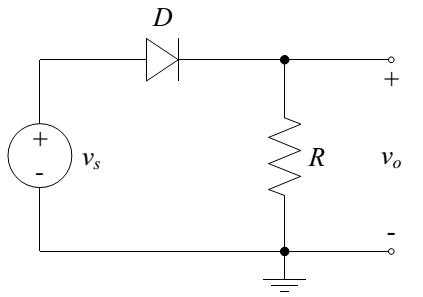
\includegraphics[width=6cm]{task1_1.png}
        \captionof{figure}{The circuit in Task 1.1}
    \end{figure}

\subsection*{1.2}
    %Observe  the  input  signal  vs and  output  signal  vo using  the  oscilloscope.  
    %Determine  the voltage drop across the diode.

    The input signal, v$_s$, and the output signal, v$_o$, were observed by using the oscilloscope.\\

    %FIG2 OSCILLOSCOPE SHOWING INPUT AND OUTPUT SIFNALS
    \begin{figure}[h!]
        \centering
        %\includegraphics[width=5cm]{task1_2.png}
        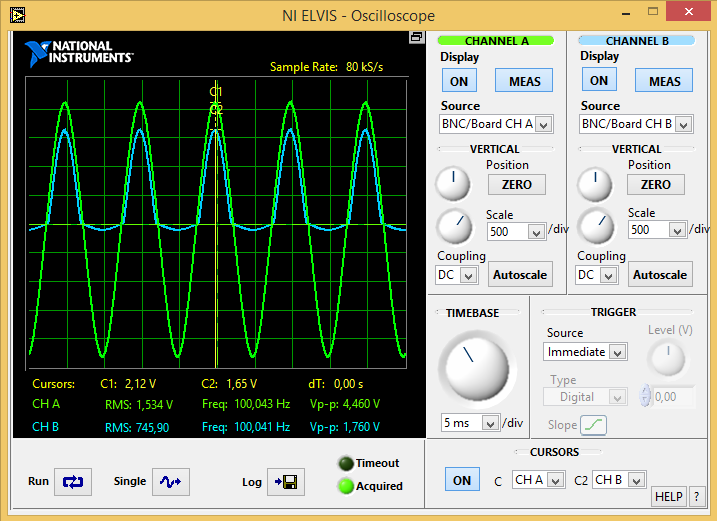
\includegraphics[width=10cm]{task1_1b.png}
        \captionof{figure}{The oscilloscope for the analysis of the circuit in figure 1}
    \end{figure}

    Using values read from the oscilloscope seen in figure 2, the voltage drop across the diode was determined using the following formula.

    $$V_d = V_{s,peak} - V_{o,peak} = 2.12 \ V - 1.65 \ V = 0.47 \ V$$
\pagebreak
\subsection*{1.3}
    %Modify the rectifier circuit as shown below:

    The half-wave rectifier circuit was modified by adding a capacitor C in parallel with resistor R as shown in figure 3.

    %FIG3 CIRCUIT DIAGRAM OF THE MODIFIED HALF-WAVE RECTIFIER
    \begin{figure}[h!]
        \centering
        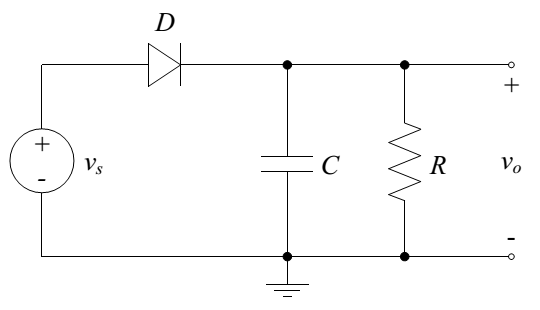
\includegraphics[width=6cm]{task1_3.png}
        \captionof{figure}{The circuit in task 1.3.}
    \end{figure}

\subsection*{1.4}
    %For each of the following capacitance values C = 0.22 µF and C = 1 µF observe the input
    %and  output  signals  using  the  oscilloscope.  Determine  the  value  of  the  ripple  voltage  in
    %each case. 
    
    The input signal, v$_s$, and the output signal, v$_o$, were observed using the oscilloscope for the following capacitance values C = 0.225 $\mu$F and C = 0.984 $\mu$F and the ripple voltage was determined.\\
    
    The theoretical value for the ripple voltage is determined with the discharging formula for a capacitor in parallel with a resistor:
    $$ V_r = V_p - V_p \ e^{-T/RC} =  V_p - V_p \ e^{-1/fRC}$$ 
    
    The peak voltage after the diode must also be recognized were that voltage is the peak voltage over the capacitor and the output:
     $$ V_p = V_{p,Input} - V_d = 2.22 \ V - 0.47 \ V = 1.75 \ V$$.

\subsection*{1.4.1: Capacitor value 0.225 \textbf{$\mu$}F}    
    \begin{figure}[h!]
        \centering
        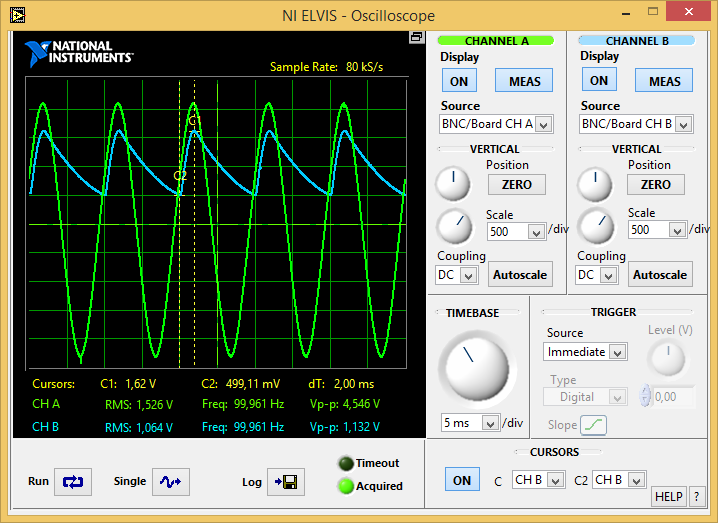
\includegraphics[width=10cm]{task1_4_022uF.png}
        \captionof{figure}{The oscilloscope for the circuit in task 1.3 with the capacitor value at $0.225 \ \mu F$ }
    \end{figure}
    
    From figure 4 the ripple voltage for the diode can be calculated from the measured data: $$ V_{r,0.225 \ \mu F} = 1.62 \ V - 0.499 \ V = 1.12 \ V $$
     The theoretical value is then calculated with the formula for a discharging capacitor:
    
     $$ V_{r,0.225 \ \mu F} = 1.75 \ V - 1.75 \ V \ e^{-1/(100 \cdot 32.5k \cdot 0.225 \ \mu F)} = 1.30 \ V $$\\
\pagebreak
\subsection*{1.4.2: Capacitor value 0.984 \ \textbf{$\mu$}F}    

    \begin{figure}[h!]
        \centering
        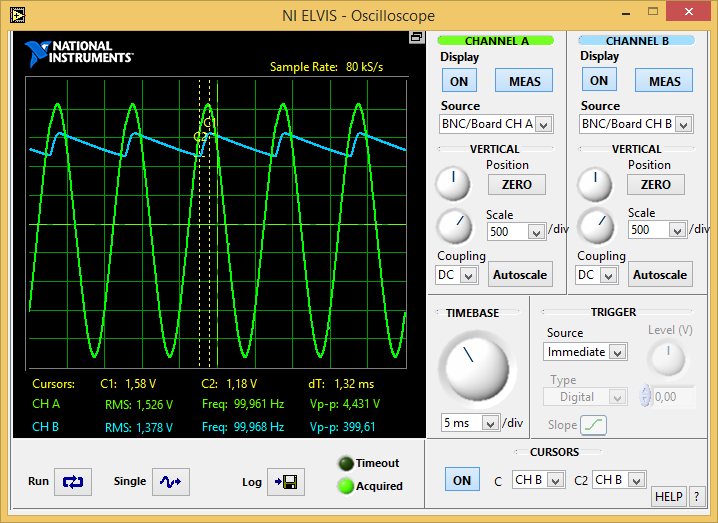
\includegraphics[width=10cm]{task1_4_1uF.png}
        \captionof{figure}{The oscilloscope for the circuit in task 1.3 with the capacitor value at $0.984 \ \mu F$ }
    \end{figure}
    
    From figure 5 the ripple voltage for the diode can be calculated from the measured data: $$V_{r,0.984 \ \mu F} = 1.58 \ V - 1.18 \ V = 0.40 \ V $$
     The theoretical value is then calculated with the formula for a discharging capacitor:
    
     $$ V_{r,0.984 \ \mu F} = 1.75 \ V - 1.75 \ V \ e^{-1/(100 \cdot 32.5k \cdot 0.984 \ \mu F)} = 0.47 \ V $$


    

\subsection*{1.5}
    %Compare  the  values  of  the  ripple  voltages  obtained  experimentally  with  the  theoretical
    %ones. 
    
       % Table generated by Excel2LaTeX from sheet 'Sheet1'
      % Table generated by Excel2LaTeX from sheet 'Sheet1'
   \begin{table}[htbp]
     \centering
       \begin{tabular}{c|c|c|c}
       Capacitor Value [$\mu F$] & Measured ripple voltage [V] & Theoretical ripple voltage [V] & $\Delta V_r$ [V] \\
       \hline
       0.225         &     1.62 - 0.499 = 1.12        & 1.30 & 0.18 \\
       0.984         &     1.58 - 1.18 = 0.40         & 0.47 & 0.07 \\       
       \end{tabular}%
       \caption{Comparison between theoretical and measured ripple voltage}
     \label{tab:addlabel}%
   \end{table}%

The theoretical values and the measured values match very well and the error is not significant. The difference in between the theoretical and the measured values are due to the instruments used, the Elvis.
    



